\documentclass[letterpaper]{sig-alternate}

\usepackage{hyperref}

\pdfpagewidth = 8.5in
\pdfpageheight = 11in

\widowpenalty=3000

\usepackage[factor=250,spacing=true]{microtype}

\begin{document}
\conferenceinfo{RecSys '14}{October 6--10, 2014, Foster City, Silicon Valley, USA}
%\CopyrightYear{2007} % Allows default copyright year (20XX) to be over-ridden - IF NEED BE.
%\crdata{0-12345-67-8/90/01}  % Allows default copyright data (0-89791-88-6/97/05) to be over-ridden - IF NEED BE.

\title{Evaluating Recommender Behavior For New Users}

\numberofauthors{2}

\author {
\alignauthor
Daniel Kluver\\
\affaddr{GroupLens Research}\\
\affaddr{Department of Computer Science and Engineering}\\
\affaddr{University of Minnesota}\\
\affaddr{Minneapolis, MN 55455 USA}\\
\email{kluver@cs.umn.edu}
\alignauthor
Joseph A. Konstan\\
\affaddr{GroupLens Research}\\
\affaddr{Department of Computer Science and Engineering}\\
\affaddr{University of Minnesota}\\
\affaddr{Minneapolis, MN 55455 USA}\\
\email{konstan@cs.umn.edu}
}

\maketitle
\begin{abstract}

  The new user experience is one of the important problems in recommender systems.
  Past work on recommending for new users has focused on the process of gathering information from the user.
  Our work focuses on how different algorithms behave for new users.
  We describe a methodology that we use to compare representatives of three common families of algorithms along eleven different metrics.
  We find that for the first few ratings a baseline algorithm performs better than three common collaborative filtering algorithms.
  Once we have a few ratings, we find that Funk's SVD algorithm has the best overall performance.
  We also find that ItemItem, a very commonly deployed algorithm, performs very poorly for new users.
  Our results can inform the design of interfaces and algorithms for new users.

\end{abstract}

%TODO: update these things.
% A category with the (minimum) three required fields
\category{H.3.3}{Information Search and Retrieval}{Information filtering}

%TODO: update these things.
\terms{Algorithms, Measurement}

%TODO: update these things.
\keywords{Recommender Systems, Evaluation, Profile Size, New User Experience, New User Problem, User Cold Start}

\section{Introduction}

  % new user experience is only chance to make all important first impression
  One of the important problems in recommender systems is the new user experience.
  If the system cannot provide a good user experience, then new users are likely to leave and not return.
  Even if the system can make accurate recommendations, accuracy alone is not enough to make a good first impression.
  If the system only recommends items the user has seen, then the user may see no value in the system and leave.
  Alternatively, if the system only recommends obscure items, then the user will have no way to know if the recommendations are worth taking.
  This problem is made more complex by how little information we have about new users.
  
% one important trait is trust.
    % trust is complex
    % matching user's experience is probably important.
  %One important part of how the user interacts with a recommender system is how much the user trusts the recommender system.
  %The more the user trusts a recommender system, the more the user can take advantage of it.
  %If the user doesn't trust a recommender system, the system can be of no value to the user.
  %Building trust with the user is therefore an important part of the new user experience.
  %Past work has shown that one of the strongest factors in the formation of trust is how much the system's recommendations match the user's knowledge \cite{wangAttributionOfTrust}.
  %For new users this can easily take the form of recommending items that the user has already seen.
  %TODO: I kinda of want to cut this. I want to talk about this theme, but I don't actually know where it fits in.

  % past work tends to focus on the algorithm side, the algorithm side of this problem is cold start.
    % Small DATA TENDS TO IMPLY BAD RESULTS.
    % cold start algorithms is a larger problem
    % cold start algorithms tend to use extra information to help improve Early performance.
    % we only look at user cold start as it is ubiquitous.
  Past work on new user experience in recommender systems has tended to focus on the `cold start problem'.
  Cold start refers to the problem that no algorithm can make highly personal recommendations with very limited amounts of information.
  Unfortunately this means that regardless of the algorithm, no recommender system can make high quality recommendations for users who are still joining the system.
  
  % One common new user strategy is to have a special data collection mode.
  % collect ratings fast to get over a precived ``bad period''
  % work on this focuses on how to collect useful ratings.
  % (framework from decision tree work)
 
  The most studied strategy for gathering more information for new users is to include a new user rating survey.
  Systems that utilize this practice do not allow their users to receive recommendations until some fixed number of ratings have been entered.
  The idea is that after enough ratings have been entered, the predictions will be `good enough'.
  This idea has been explored by many authors; most consider a system in which the user is presented with a list of items and asked to rate items until they have enough ratings.
  For a good discussion of prior work in this direction see \cite{adaptiveBootstrapping}.

  % One promising approach is to let user control interaction
  % user or system driven control.
  % promising, we don't know much about follow up.
  %One promising approach to the new user rating survey is to have users control which movies they rate.
  %This was pioneered by McNee et al., who looked at comparisons between user driven and system driven new user surveys \cite{mcneeInterfaces}.
  %They found that users who were in control of the items they rated made fewer ratings, but that the profiles they created were more useful in predicting the user's future ratings.
  %Interestingly, while these users took more time to create their profiles, they were just as likely as other users to report that the sign up was short.
  %While these results are quite promising, to our knowledge no follow up work has been done to explore these issues further.
  %This goes to show, however, that the new user experience is a complicated issue and novel strategies may yet prove to be the best solution.

  % bridge from past work to our work.
    % point out holes (evaluating standard algorithms for little to no ratings, wholeistic evaluation)
    % point out that other approaches than smart object ordering exist, and we need to be able to compare.

  While past work has carefully covered the new user rating survey, it has not carefully evaluated which algorithm is best at recommending to new users.
  The new user survey work sidesteps this issue by assuming that the user will receive no personalization until the survey is complete.
  Even for systems with a new user survey, carefully choosing algorithms for new users may be very important.
  Users fresh out of the new user survey will still have far fewer ratings than the average user of the recommender system.
  Different algorithms may provide very different experiences for these users, even if they give very similar results for the average user.
  
  The ideal way to study this issue would be a live study with real people who are new to a recommender system.
  Users could be randomly assigned an algorithm and then surveyed after a random number of ratings to establish what they thought of the new user experience. 
  Unfortunately, there are many algorithms and new users are a scarce resource.
 
  Fortunately, there has been a growing trend in recommender system research to perform multiple metric offline evaluations of recommender systems.
  This work comes out of a pushback against early recommender evaluations which only evaluated recommenders in terms of their predictive accuracy \cite{accurateIsNotEnough}.
  The response of this pushback has been the generating of many different metrics which allow us to more carefully understand the separate aspects of a recommender's output \cite{LathiaTemporal, CremonesiTopN, zieglerDiversity}.
  %TODO: I want to cite more papers here, I don't think I have good ones either. Joe would probably know.
  This strategy allows us to dig much deeper into the differences between algorithms, looking past simple measures of accuracy to more meaningful dimensions such as how novel the recommendations are, or how frequently the recommendations change for any user.
  This allows us to capture the qualitative tradeoffs between algorithms which are otherwise quite similar, which helps us choose algorithms that are better suited for a particular domain.

  In this work we combine these two streams of research: new user experience research and multiple metric algorithm evaluation.
  Our goal is to understand the differences between algorithms for new users, especially how these algorithms respond to different amounts of information.
  By using multiple metrics we can understand not just what algorithm is best in terms of absolute performance, but also gain a more nuanced understanding of the qualities of different algorithms' recommendations.
  %Furthermore, we do not seek to find the algorithm that scores best on some metric of choice, instead, we seek to form a complete understanding of the differences between algorithms for cold start use.

  We structure our work around the following research question:
  \begin{itemize}
    \item RQ1: How do algorithms behave for users with few ratings?
  \end{itemize}
  Algorithm behavior is a very broad subject.
  We will look at three distinct sub-questions to help capture algorithm behavior.
  %We will look at three distinct ways to quantify the behavior of a recommender system. each of which will lead to multiple metrics.

% RQs
    % RQ1 How do the behavior of different algorithms change with the number of ratings?
      % Explain that there are a lot of different ways to measure algorithm behavior.
        % Predictive accuracy, commonly measured with MAE or RMSE
          % coverage
        % Value of recommendations, tradidionally done with metrics from information retrieval such as precision, recall, MAP, etc. These algorithms try to measure ...
          % cite the John/Joe paper (RMSE is not enough)
          % cite the paper cited by 10 is enough
          % topN RMSE
        % There are many properties of recommenders that are (find words here)
          % popularity
          % diversity
          % spread
      
  \begin{itemize}
  \item RQ1.a: How well can different algorithms predict the future ratings of new users?
  \item RQ1.b: How well can different algorithms rank and recommend good items to new users?
  \item RQ1.c: How do algorithms behave as measured by other metrics, such as popularity and diversity, for new users?
  \end{itemize}

  We will answer these questions by developing an evaluation framework that can be used to understand how algorithms perform for new users.
  This framework will compare algorithms on eleven different metrics to allow a more complete understanding of the differences between algorithms.
  We will then use this framework to study how three common algorithms behave for new users.
  Finally, we will draw conclusions from our evaluation and outline directions for future work.

\section{Methodology}
\label{sec:methodology}
  % (high level description/restatement of approach) To answer our research questions we will various metrics of recommenders in an offline setting simulations users as they join the system.
    % maybe hit some limitations
    % motiviate _why do a simulation_ (a lot of metrics we want to try)

  Ideally we would measure new user experience with a live survey on users who are just joining a recommender service.
  Because new users are a scarce resource we opt to first explore the new user experience in an offline setting.
  This allows us to test many more profile sizes and algorithms much faster than an online study.
  We will adapt the standard train and test methodology so that test users have only a specified number of training ratings.
  By running this approach for various profile sizes we can generate plots of performance against profile size.
  This lets us understand both how the algorithms compare on these metrics, and how the algorithm performance changes with the number of ratings provided.

  This, or a similar technique, has been used by previous authors to make plots of metric values over profile size \cite{DrennerInitialExperiance, TenIsEnough, AdaptiveBootstrap, LathiaTemporal}.
  Past work used these plots to establish that more ratings lead to better results.
  We take this technique farther and develop a much more nuanced understanding of the different algorithms, and how they compare for different profile sizes.

  Our approach is related to the temporal evaluation methodology, in which a recommender is repeatedly trained on all ratings up to a point in time, and then tested using the next ratings to be made for each user.
  Temporal evaluations have been used in the past to evaluate how the list of recommended items change as users enter more ratings into the system \cite{LathiaTemporal}.
  While the output of a temporal evaluation can be very similar to our own, the methodologies have some key differences.
  Where a temporal evaluation is designed specifically to consider the order in which users make ratings, our methodology is designed to try to eliminate this ordering effect from our consideration of the algorithm's behavior.

  As mentioned earlier, many recommender systems use a new user survey to collect the first user ratings.
  These ratings are different than normal user ratings.
  As we explain shortly, our methodology uses randomization in key places to remove this ordering effect.
  This allows us to better capture the underlying algorithm performance on ``normal'' user data.
  While this makes our methodology unsuited for applying temporal metrics, it allows us to separate an algorithm's behavior from how ratings are collected for new users.
  We feel that this is better given the limitations of our dataset, and our focus on the algorithm, rather than how ratings are collected.

  \subsection*{Algorithms}
  % algorithms (discuss tuning of algorithms per algorithm?)
  % motivation for algorithm selection
  % list algorithms 

  We seek to develop an understanding of how a range of different standard algorithms perform for new users.
  Rather than picking advanced algorithms that are tuned for new user performance, we decided to first understand how representatives of three common types of algorithms perform.
  Therefore we will compare UserUser\cite{resnick1994grouplens}, ItemItem\cite{sarwar2001item}, and Simon Funk's SVD\cite{funk_netflix_2006} against two simple baseline algorithms.
  
  Due to the low profile sizes involved in our evaluation, not every algorithm was able to make predictions for every user-item pair.
  In these cases, we use the UserItemBaseline prediction as a fallback.
  This ensured that our prediction based metrics were always evaluated over the same number of items.
  We found this unnecessary for recommendations as each algorithm was able to make a complete recommendation with only one rating.
  Therefore we form recommendations as the top 20 items that the algorithm was able to predict which were not in the training set.
  More information about these algorithms can be found in table \ref{tbl:algo}.
  Code for our evaluation, using the Lenskit evaluation framework \cite{lenskit} is available at \url{https://bitbucket.org/kluver/coldstartrecommendation}.
  
  \begin{table}[ht!]
    \centering
    \begin{tabular}{|p{6em}|p{18em}|}
      \hline
%      Algorithm          & Algorithm description \\\hline
      ItemBaseline       & Item's average rating, with mild bayesian damping towards the global mean \cite{funk_netflix_2006}. \\\hline
      UserItem\-Baseline & ItemBaseline adjusted by the user's average offset from the ItemBaseline. Mild bayesian damping is applied \cite{funk_netflix_2006}. \\\hline
      UserUser           & User based nearest neighbor collaborative filtering \cite{resnick1994grouplens} with a neighborhood size of 30 and ratings normalized by subtracting the UserItemBaseline score. \\\hline
      ItemItem           & Item based nearest neighbor collaborative filtering \cite{sarwar2001item} with a neighborhood size of 30 and ratings normalized by subtracting the ItemBaseline score.   \\\hline
      SVD                & Simon Funk's SVD based collaborative filtering approach \cite{funk_netflix_2006} with 30 features and 150 training iterations per feature. \\\hline
    \end{tabular}
    \caption{Summary of algorithms.}
    \label{tbl:algo}
  \end{table}

  \begin{table*}[ht!]
    \centering
    \begin{tabular}{|p{7.5em}|p{21em}|p{7em}|p{12.5em}|}
      \hline
      Metric & Description & Range & Preferred direction\\\hline
      \hline
      \multicolumn{4}{|c|}{{\bf Accuracy and Ranking Metrics}} \\\hline
      RMSE                   & Standard prediction accuracy metric \cite{handbook}. & 0 to 5 stars & Smaller is better. \\\hline
      nDCG                   & Standard ranking quality metric \cite{handbook}.     & 0 to 1       & Larger is better.  \\\hline
      \hline
      \multicolumn{4}{|c|}{{\bf Monotonic Recommendation Metrics}} \\\hline
      Precision@20           & Count of recommended items in the test set and rated 4.0 or higher\footnotemark[1] \cite{handbook}.   & 0 to 1       & Larger is better.  \\\hline
      MAP@20                 & Average of precision at each rank one through twenty \cite{manning2008introduction}.                  & 0 to 1       & Larger is better.  \\\hline
      Fallout@20             & Count of recommended items in the test set and rated 2.0 or lower\footnotemark[1] \cite{TenIsEnough}. & 0 to 1       & Smaller is better. \\\hline
      MeanRating@20          & Average rating of recommended items that are in the test set.                                         & 0 to 5 stars & Larger is better.  \\\hline
      RMSE@20                & RMSE computed only over those items that were recommended.                                            & 0 to 5 stars & Smaller is better. \\\hline
      \hline
      \multicolumn{4}{|c|}{{\bf Non-monotonic Recommender Metrics}} \\\hline
      SeenItems@20           & Count of recommended items in the test set. & 0 to 20 items & Moderate values are better. \\\hline
      Average\-Popularity@20 & The average number of users in the training set that have seen recommended items \cite{zieglerDiversity}.& 1 to 6000 users & Moderate values are better. \\\hline
      AILS@20                & The average pairwise similarity between recommended items \cite{zieglerDiversity}.                       & -1 to 1         & Moderate values are better. \\\hline
      Spread@20              & The Shannon's entropy of the distribution of recommended items for users in the test set.                & 0 to 12 bits    & Moderate values are better. \\\hline
    \end{tabular}
    \caption{Summary of metrics}
    \label{tbl:metrics}
  \end{table*}

  
  % evaluation and code to run these algortihms available at.
  % citations and lenskit info
  Each algorithm was tuned based off of Ekstrand's 2012 evaluation \cite{ekstrand2012recommenders}.
  Since this evaluation is on a different dataset (MovieLens 10M vs. MovieLens 1M), we performed minor tuning using the Ekstrand's values as a starting point.
  We tuned based on RMSE performance.
  While tuning, we found that the previous damping parameter used for the baselines to be too large.
  We found that a value of 5 gave much better results for new user recommendation.
  Our key results are not sensitive to minor changes of algorithm parameters.  

  \subsection*{Metrics}


  We present results from eleven metrics.
  As has been seen in previous studies \cite{herlockerEvaluating} we find that some of are metrics are redundant.
  Future work should be able to use a smaller list of metrics.
  The metrics are described in table \ref{tbl:metrics}.
  We split our metrics into three groups roughly along our three sub research questions.
  
  \paragraph{Accuracy and Ranking Metrics}
  {\bf RMSE} and {\bf nDCG} evaluate the recommender based on its prediction for each item.
  These evaluate the accuracy of the predictions and the ability of the recommender to rank the list of all items.
  We find that these two metrics perform quite similarly in our evaluation.

  \footnotetext[1]{We also tried 5.0 and 1.0 as cutoffs respectively, and found no meaningful difference.}\addtocounter{footnote}{1}

  \paragraph{Monotonic Recommendation Metrics}
  %TODO: daniel comment: check for consistency with the user vs. users.
  These metrics evaluate the top 20 recommendations produced by the recommender.
  The choice of 20 items for the evaluations was arbitrary, testing with other values showed similar results, except on one metric.
  This issue will be addressed later in the results section.
  We refer to these as monotonic metrics as there is a clear good direction for the metric.

  {\bf Precision@20}, {\bf MAP@20}, and {\bf Fallout@20} are standard information retrieval metrics which measure the quality of the recommendations.
  As we show later, these metrics were not useful for our evaluation.
  Therefore, to help understand the quality of our recommendations, we also include MeanRating@20, and RMSE@20.

  {\bf MeanRating@20} tries to establish how much users like their recommendations by measuring users average satisfaction with recommended items based on withheld ratings.
  {\bf RMSE@20} accompanies this metric and lets us know if the recommended items are likely to be incorrectly predicted. 
  This can help us understand why an algorithm scores well on MeanRatings@20.  
  
  \paragraph{Non-monotonic Recommendation Metrics}
  {\bf SeenItems@20}, {\bf AveragePopularity@20}, {\bf AILS@20}, and {\bf Spread@20} are all non-monotonic measures of the user's recommendations.
  These metrics are harder to apply than the monotonic measures of recommendation quality.
  Unlike the previous metrics, we expect that users will be most satisfied by moderate values of these metrics, and that both extremes can lead to a negative user experience.

  We use these metrics as they can help us understand important properties of how users perceive their recommendations.
  As mentioned in the introduction the number of recommended items that the user has seen (estimated by {\bf SeenItems@20}) can have a major impact on how much users trust the recommendations.
  If an algorithm recommends too few items that the user has seen then we expect the user will have trouble evaluating if the recommendations are trustworthy.
  Too many, and the user may feel that the recommendations are not interesting or useful.
  Unfortunately, without more research on these metrics to establish a mapping between user satisfaction and metric values we will have to rely on educated guesses to establish which values for these metrics are too extreme.

  {\bf AveragePopularity@20} is a crude metric of how novel the recommendations are to the user \cite{zieglerDiversity}.
  Broadly speaking, we expect users will prefer recommendation lists containing more novel (less popular) items.
  However, if the recommended items are too novel the user is unlikely to have heard of the items and will have no point of reference in understanding their recommendations.

  Past work has shown that users like their recommendations to be more diverse \cite{zieglerDiversity, martijnDiversity}.
  The belief is that by providing more diverse lists we are giving the user a larger range of items to choose from.
  This can make choosing an item easier as the user is less likely to have to compare very similar options.
  It has also been shown, however, that too much diversity can lead to less user satisfaction \cite{zieglerDiversity}.
  This is probably due to a tradeoff between how diverse a list is and how well it captures a user's tastes.
  At some point, a list cannot become more diverse without including items that do not interest the user.
  We will measure diversity with the {\bf AILS@20} metric.

  The {\bf AILS@20} metric is based on the Intra-List Similarity (ILS) metric introduced by Ziegler et al \cite{zieglerDiversity}.
  AILS@N is simply a rescaling of ILS to be scale free with regards to N, this was done to make the metric easier to interpret, by putting it on the same scale as similarity values.
  We used the same item similarity metric for AILS@20 as we used in the ItemItem recommender.

  The {\bf Spread@20} metric is designed to measure how well the recommender spreads its attention across many items.
  We expect that algorithms with a good understanding of its users will be able to recommend different items to different users.
  Like diversity, however, we expect that it is not possible to reach complete spread (recommending each item an equal number of times) without making avoidably bad recommendations.
  When Spread is large we know that the recommender is recommending many items with a relatively even distribution.
  When Spread is small, the recommender is focusing on a small set of items which it recommends to every user.
  In this way spread is related to item coverage metrics.
  Spread however looks at how often each item is recommended, not just whether or not it is recommended.

  Spread is computed by computing recommendations for each test user.
  Let $C(I)$ be the count of how many times item $I$ showed up in the recommendations.
  Let $P(I) = C(I) / \sum_I C(I)$ be the probability that a random recommendation is for item $I$.
  We define spread as the Shannon's entropy of $P(I)$, $Spread = -\sum_I P(I) \log(P(I))$.

  \paragraph{Expectations about algorithm performance}
  % provide expectations.
  We expect that the ItemBaseline algorithm will have approximately constant performance on all metrics.
  Since the ItemBaseline is such a simple algorithm we expect that any reasonable algorithm should be able to do better than it.
  That said, we expect the improvement over the ItemBaseline to be gradual, with larger improvements only happening with more data.

  The UserItemBaseline should only differ from the ItemBaseline for metrics that use the prediction value.
  For all other metrics these two provide the same responses, and we will only report results for the ItemBaseline.
  As the UserItemBaseline is still quite a simple baseline, we expect that the non-baseline algorithm will beat this baseline as well given enough ratings.
  
  We expect that the baseline algorithms will provide the most popular recommendations, with the least diversity, and the least spread.
  Any personalized algorithm should be able to make more nuanced recommendations than simply recommending the best rated items, which should translate as gains on these metrics.
  Furthermore, we expect that as an algorithm learns more about the user it should decrease in popularity, and increase in diversity, and spread, as it becomes able to make more personal and nuanced recommendations.


  \subsection*{Dataset}
  % dataset
    % # user
    % # items
    % distributions of # ratings per user (important: min 20)
    % establish range of evaluation.

  For this evaluation we will use the MovieLens 1M dataset\footnote{\url{http://grouplens.org/datasets/movielens/}}.
  This dataset contains 1 million ratings from 6000 users on 4000 movies.
  
  These ratings were collected from the MovieLens system, which requires 15 ratings in a new user survey before users can enter the system.
  To the best of our knowledge, at the time this data was collected the new user survey preferred items that were very popular.
  We will randomize the order of the ratings to try to avoid measuring the effect of these initial ratings, and instead focus on the algorithm's performance on normal ratings.
  
  Each user in the dataset has at least 20 ratings.
  Therefore we will evaluate user profiles with up to 19 ratings.
  This will allow us to ensure that each user in the dataset has at least one test rating.

  
  \subsection*{Evaluation Procedure}

  % subsampling strategy
  % describe normal crossfold solution
  The natural way to perform this evaluation is with a modified user crossfold strategy.
  The normal five-fold cross validation strategy splits the users into five groups.
  In each of five folds all ratings from four of the groups will be kept in the training set, and then some subset of the ratings from each user in the fifth group will be set aside for the test set.
  The selection of a test set can be random to avoid any possible ordering effects in the data due to a new user rating strategy.
  To understand how metrics change with a different number of users we can simply generate separate random crossfolds for each simulated profile size.
  At each crossfold we include only a constant number of training ratings for each test user, ensuring that all test users have the specified profiles size.
  
  % describe issues with solution
  Unfortunately, we found that this strategy causes biases in our evaluation.
  In particular, this strategy led to the size of the test sets changing as a function of the simulated profile size.
  As we kept more ratings for the training set, we would have fewer ratings in the test set.
  This biased our results; some metrics such as nDCG proved to be sensitive to the size of the test set.
  As we compared different profile sizes we would see trends that were solely a property of the changing test size.
  
  % describe our crossfold then subsample solution.
  Our solution to this bias is to subsample from an existing crossfold.
  To generate training and test sets for different number of ratings from 1 to 19, we first generate a set of test and training splits so that test users have 19 training items using the crossfold strategy outlined above.
  Then, to generate any other number of ratings, we randomly downsample the 19 item training set.
  This allows us to generate training sets with a given number of ratings for test users, such that each profile size is evaluated with the same test set.


 % Prediction accuracy
\begin{figure*}[ht!]
  \centering
  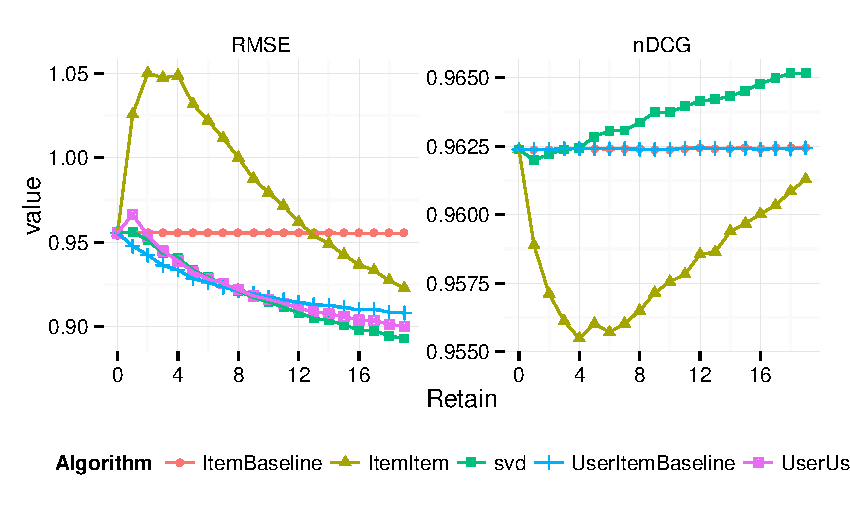
\includegraphics[width=0.75\linewidth]{../lenskit/output/ekstrandTuned20/accuracy.pdf}
  \caption{Accuracy and Ranking Algorithms}
  \label{fig:rmse}
  \label{fig:ndcg}
\end{figure*}


\section{Results}

  Using the methodology described in section \ref{sec:methodology} we generate plots for each metric showing how the five algorithms perform versus simulated profile size.


  
\subsection*{Accuracy and Ranking Metrics}

\vspace{-1.5em}
 
    % RMSE plot
    % point out error bars etc.
    % explain / interpret plot
  \paragraph{RMSE}
  Figure \ref{fig:rmse} shows how accurate our algorithms are as measured by RMSE.
  UserUser, and SVD both behaved essentially as expected.
  SVD shows no improvement with only one rating, and UserUser actually gets worse with the first rating.
  Other than that, these algorithms outperform ItemBaseline.
  Interestingly, UserItemBaseline outperforms both algorithms until around 8 ratings, at which point both algorithms start to perform better.
  Given the size of the differences between UserItemBaseline, UserUser, and SVD we conclude that all three are equally accurate for new users.
  That such a simple algorithm can outperform more complicated algorithms for small profile sizes suggests that recommending for users with very few ratings is a hard problem.
  
  ItemItem performs quite poorly for new users.
  Until we have 13 ratings, ItemItem is less accurate than the ItemBaseline.
  In fact, for the first two ratings ItemItem appears to perform \emph{worse} as more ratings are added.
  This trend is a result of the limited coverage of the ItemItem algorithm.
  Considering the accuracy of RMSE on only those items where it makes a personalized prediction, it shows a monotonic increase in accuracy similar to the other algorithms.
  However, for small rating counts ItemItem can only predict for some percent of the items (around 60\% for users with two ratings, and around 75\% for users with four ratings).
  Because of this, many of the predictions come from the better performing UserItemBaseline.
  As we get our first few ratings, the predictions become less likely to be from the UserItemBaseline, leading to an artificial upward trend in RMSE.
  
\footnotetext[3]{We do not plot UserItemBaseline here as it is equivalent to ItemBaseline on this metric.}

  % Recommendation quality metrics
    % NDCG
  \paragraph{nDCG}
  Figure \ref{fig:ndcg} shows the algorithms performance on the nDCG metric.
  The results for nDCG are very similar to the RMSE results.
  Both UserUser and SVD take an initial hit to accuracy at the first rating.
  This time UserUser takes much longer to recover and only beats the baseline after around 12 ratings.
  Again ItemItem performs quite poorly.
  This leaves SVD performing the best, passing the baseline after about 3 ratings.
  Again we find that our best algorithm for the first few ratings is our baseline.
  
    % MAP, precision, fallout plots 
    % explain results from MAP and precision
    % explain recall results
    % recall results, strangeness and popularity


\subsection*{Monotonic Recommendation Quality Metrics}

\vspace{-1.5em}

\begin{figure*}[ht!]
  \centering
  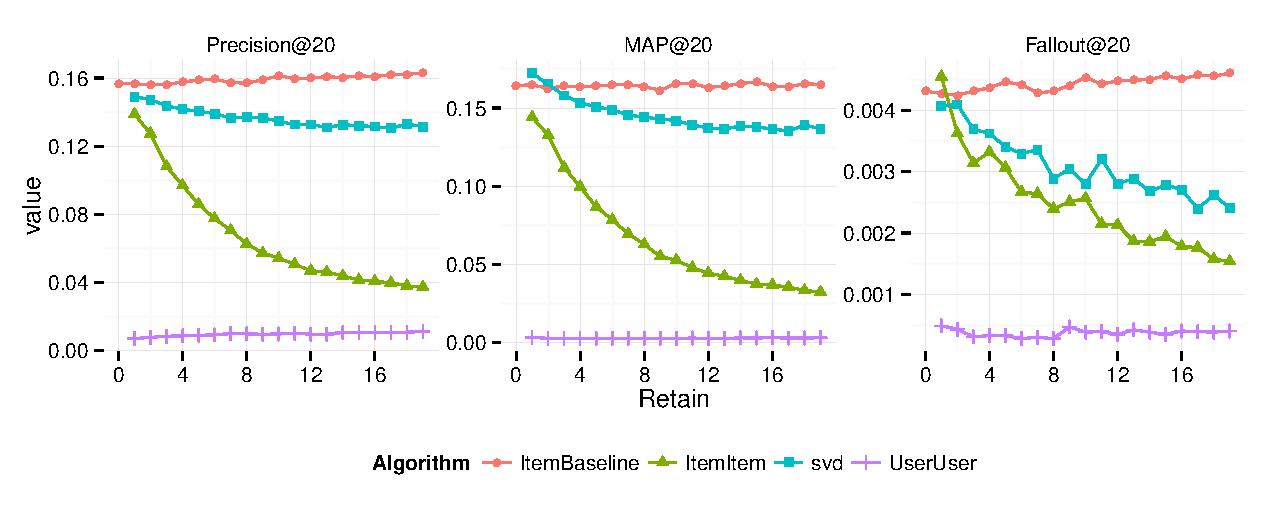
\includegraphics[width=\linewidth]{../lenskit/output/ekstrandTuned20/TopNPrecision.pdf}
  \caption{Information Retrieval Recommendation Quality Metrics}
  \label{fig:map}
\end{figure*}
%
\paragraph{MAP@20, Precision@20, Fallout@20}
  Figure \ref{fig:map} shows MAP@20, Precision@20, and Fallout@20.
  All three metrics show essentially the same trend, UserUser gets the lowest score, the baseline get the highest score.
  On both MAP@20 and Precision@20, SVD gets a higher score than ItemItem throughout, performing almost as well as the baseline.
  On Fallout@20 ItemItem and SVD perform about as well as each other, with SVD showing a very slight lead.
  We also tested recall and mean reciprocal rank metrics, but found them to exhibit the same trend, so they were not explored further.

  This result is rather strange as MAP and Precision are metrics where larger scores imply better performance, whereas Fallout is a metric where larger scores imply poor performance.
  Therefore we would not expect to see rank equivalent behavior from these metrics.
  Unfortunately this means that these metrics contradict each other.
  One possible reason for this is that these topN metrics are known to be biased toward algorithms that recommend more popular items \cite{bellogin}.
  Looking forward to the average popularity (figure \ref{fig:pop}) of recommended items, we see that the average popularity of the recommendations closely replicates the previous three plots.
  As a result of this, we discard these metrics, and consider less biased metrics to help us analyze the quality of the recommendations.

  % TopN average rating / topn rmse
    % interpret graph and reason about what it means about quality

\begin{figure*}[ht!]
  \centering
  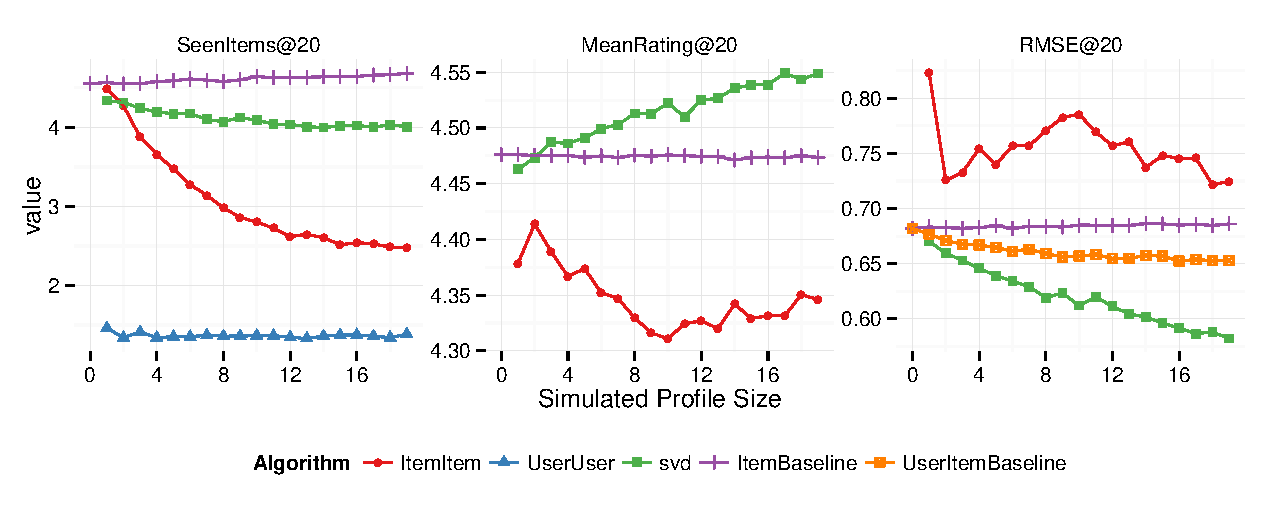
\includegraphics[width=\linewidth]{../lenskit/output/ekstrandTuned20/rmse_20.pdf}
  \caption{Recommendation Quality Metrics}
  \label{fig:topN.rmse}
\end{figure*}

  \paragraph{SeenItems@20}
  We address this non-monotonic metric out of turn here as it provides important context for the next two metrics.
  The first graph in figure \ref{fig:topN.rmse} shows the average number of items in the top 20 recommendations for each algorithm that were also in the test set.
  The average number of test set items in recommendations shows a similar trend to the MAP and precision metrics, with UserUser getting by far the fewest seen items, and the baseline getting the most.
  As UserUser gets less than one seen item on average we found that UserUser was not appropriate for the MeanRating@20 and RMSE@20 metrics.
  In particular, we found that the UserUser results for these metrics are highly sensitive to recommendation list size.
  Because of this issue we will not include UserUser in our next two metrics and consider the next two metrics inconclusive for UserUser.
  That said, we consider the small number of seen items to be a bad result for UserUser.
  Put simply, if we cannot reliably estimate if the recommendations are reasonable, how can we expect a user to do so?

  \paragraph{MeanRating@20}
  The second graph in figure \ref{fig:topN.rmse} shows the average rating for those items in the top 20 recommendations for each algorithm.
  The first thing to note about this graph is that all of these algorithms are doing a reasonable job of recommending items the user might like to watch, with all algorithms averaging above 4 stars (implying that the recommended items are, at least on average, enjoyable).
  SVD performs as expected, starting around the baseline for a few ratings, and then steadily improving to be the best algorithm after 3 ratings.
  Again, we find that ItemItem performs poorly until quite a few ratings are added, and does worse than baseline throughout.
    
\footnotetext[4]{We do not plot UserUser here as it cannot be reliably measured for this metric.}

  \paragraph{RMSE@20}
  The third graph in figure \ref{fig:topN.rmse} shows the accuracy of our algorithms on items in the top 20 recommendations.
  Not surprisingly, this figure shows the same trends as the last one, meaning that the algorithms whose recommendations were (on average) most likable, were those whose recommendations were most accurate.
  Again, SVD performs quite well, easily beating the UserItemBaseline after only 1 rating.
  
  %Interestingly, we find that all algorithms are quite a bit more accurate on the top 20 items than they are for the general item collection.
  %This is likely an edge effect, where the highest rated (5 star) items are perhaps easier to predict than other items.


\subsection*{Non-monotonic Recommender Quality Metrics}
  % Other recommender metrics
\vspace{-1.5em}
\begin{figure*}[ht!]
  \centering
  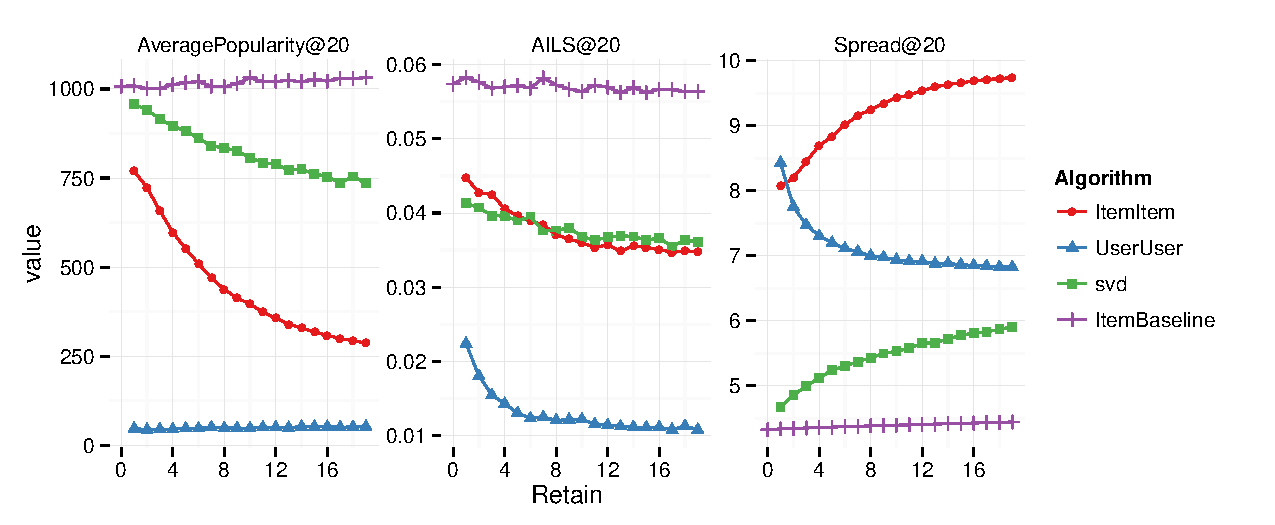
\includegraphics[width=\linewidth]{../lenskit/output/ekstrandTuned20/popdiv.pdf}
  \caption{Non-monotonic Recommendation Quality Metrics}
  \label{fig:pop}
\end{figure*}
%
  \paragraph{AveragePopularity@20}
    % popularity graph
  The first graph in figure \ref{fig:pop} shows the average popularity of items recommended by each algorithm.
  As expected the baseline algorithms makes the most popular recommendations, followed by SVD, ItemItem, and then UserUser in a distant last.
  As stated earlier, We expect that users will feel the baseline's popularity (around 1000) is too high.
  We also expect that users will perceive UserUser's popularity (around 50) as too low.
  SVD and ItemItem both seem to perform well, with SVD generating more popular recommendations than Item-Item.
  SVD and ItemItem both show a trend of decreasing popularity as more ratings are entered, suggesting that these algorithms will make more nuanced, less popular recommendations for users they know more about.
  %Interestingly, these algorithms each appear to be converging to their own separate level of popularity, which suggests that this ordering may be independent of the number of ratings.

    % diversity plot
  \paragraph{AILS@20}
  The second graph in \ref{fig:pop} shows a similar trend to the popularity trend.
  Again, we expect that the baseline, which provides the least diverse recommendations, would be perceived as not very diverse by users.
  Quite possibly due to the preference for obscure movies, UserUser seems to produce the most diverse lists of any algorithm.
  We expect that the UserUser recommendation lists might be too diverse.
  Unlike popularity, SVD and ItemItem seem to perform equivalently in terms of diversity.
  We also see that all three collaborative filtering algorithms show a trend of increasing diversity (decreasing inter-list similarity) as more ratings are entered.

  % spread plot
  \paragraph{Spread@20}
  The third graph in figure \ref{fig:pop} shows the spread of the recommendations from each algorithm.
  As expected the baseline performs worst on spread, as it recommends essentially the same items to each user.
  SVD performs mildly better than the baseline, and shows definite improvement as more ratings are added.
  UserUser and ItemItem start at around the same value as each other, however, after only two ratings they have crossed, as ItemItem quickly increases to have the highest spread of all the algorithms, and UserUser quickly decreases into second place.
  Interestingly, only UserUser shows a trend to have less spread as it learns more about the user, ItemItem and SVD both show the expected trend of increasing Spread as they learn more.
  This could be some form of a regression towards the mean, where as it learns more about users its recommendations become less personalized to the users individual quirks.
  More research will be needed to understand this trend.
  

\section{Discussion}
  % summary of results in a big old table.
    % the accuracy of svd and user-user both seemed good. item-item seemed to have trouble especially with very new users.
    % svd did quite well on our traditional topN metrics, item-item did OK, and user-user did bad., but there are flaws with these metrics.
    % on our topN RMSE item-item (again) seemed to have issues, and user-user did quite well, but the low hit rate is troubleing. 
    % again svd seems the winner here.
    % on our fluffy metrics item-item and svd seemed to do well. I might argue that item-item seemed to do better (spread, and higher throughout).
    % user-user seemed to do poor

  % what this means
    % user-user seems to be able to give accurate predictions, but seems to focus on overly obscure items in recommendation.
    % item-item seems to give not-bad recommendations, but its predictions have issues
    % based only on these results svd seems to be the best performer and is our recommendation to new systems.
    
  \begin{table}[ht!]
    \centering
    \begin{tabular}{|p{4.5em}|p{4.5em}|p{7.5em}|p{4.5em}|}
      \hline
      {\bf Algorithm} & {\bf Prediction accuracy} & {\bf Recommendation quality} & {\bf Other properties} \\\hline
      ItemItem        & Poor                      & Poor                         & Good                   \\\hline
      UserUser        & Good                      & Inconclusive                 & Poor                   \\\hline
      SVD             & Good                      & Good                         & Good                   \\\hline
    \end{tabular}
    \caption{Summary of algorithm behavior for new users}
    \label{tbl:results}
  \end{table}

  The high level results of our evaluation are summarized in table \ref{tbl:results}.
  Overall we see that SVD seems to be the best performing algorithm for cold start use.
  SVD was the only algorithm that consistently outperformed the baseline algorithms on prediction and recommendation tasks.
  ItemItem had arguably better results on the average popularity and spread metrics, indicating that it was able to find more novel items, and make a larger range of recommendations to users.
  Unfortunately, ItemItem also performed quite poorly at both prediction and recommendation, which makes it less suitable for new users.

  UserUser performed quite well at prediction, but tended to favor unpopular items in its recommendations.
  While some novelty is good, we believe that UserUser goes too far with obscure movies in its recommendations, and therefore does not make good recommendations.
  Therefore we conclude that UserUser alone is not well suited for new users.
  It is possible that careful tuning or hybridizing with another algorithm may help UserUser perform well for new users.
  Exploring this issue further is left as future work.

    % if you use a switching recommender, this methodology can help you choose when to switch.
    % non-traditional metrics can tell you more about what is going on, these seem to be more properties of the class of algo than of the data, so its worth looking at these when choosing algorithms, to find one with properties that are good for your task.
  Interestingly, we repeatedly see that for very small numbers of ratings the UserItemBaseline is our strongest algorithm, both in terms of accuracy, and recommendation quality.
  This suggests a switching strategy for live systems, in which the UserItemBaseline is deployed until a user has enough ratings, after which they are switched to a better recommender.
  The switching point between algorithms can be determined with our methodology.
  The only downside of this approach is that the baseline performed poorly on our non-monotonic metrics, which may effect users as they first join the system.
  

  % other takeaways
    % regularization
  One possible reason that the SVD algorithm performs as well as it does is the regularization built into the algorithm.
  UserUser and ItemItem algorithms have no built in method for damping their predictions towards the mean when they don't have much data.
  The regularization in the cost function of the SVD model makes it so its predictions will gradually shift away from the baseline predictions as more relevant ratings are added.
  The downside of this, however, could be the higher popularity and lower spread seen by the SVD algorithm.
  The same regularization that helps avoid making mistakes due to too little data may also prevent the algorithm from taking occasional risks on more obscure movies.
  

  % limitations and opprotunities
    % dataset limitations
      % only one domain
      % no quitters in our dataset

  One of the limitations of our work is that we only evaluated on one dataset.
  Future work should replicate our experiment on other datasets from different domains, or where ratings are collected in different ways.
  This will establish which of our results are true properties of the algorithms, and which results are specific to our dataset.

  One important issue that our methodology cannot address is that we can only compare users who have made some minimum number of ratings (20 for our dataset)
  Unfortunately, this means that we do not know if there are differences between users who do and do not survive in the system.
  This is an unfortunate side effect of insisting on a constant test set throughout the evaluation.
  More work needs to be done to understand users who only make one or two ratings to understand how they are different and discover why they leave the system.

  Nonetheless, we feel that our methodology will allow offline comparisons of many different cold start experiences.
  Our work has only scratched the surface of recommender algorithms.
  Future work can be done comparing these standard algorithms against newer algorithms such as those designed for cold start, or those designed to leverage extra non-rating information.
  More work should be done to understand how extra information about a user can effect cold start ratings.
  Our methodology can be used to measure this effect, and even establish a tradeoff between the extra information or extra initial ratings.
    % algorithm limitations
      % only covered three common families,
      % different algos tuned specifically for cold start.
      % algos that use extra data about users or about items.
    % cite the comparison work at CHI.

  % despite the limitations we were able to show differences between algorithms in a cold start situation.


\section{Conclusion}
  We find that recommending for new users is hard and none of our algorithms can reliably beat a simple baseline for users with very few ratings.
  Once the user has a small number of ratings we find that the SVD algorithm performs best.
  This result can be useful both in designing new recommender systems, and in designing novel recommendation algorithms for new users.
  We also present a methodology and list of metrics for understanding recommender behavior that can be used to extend our results to other algorithms and datasets.

\section{Acknowledgements}
  
  The authors would like to express their gratitude towards our colleagues at GroupLens research for their feedback and support while developing this work.
  We would like to specially thank Michael Ekstrand for his  important work on the Lenskit recommendation framework.
  This work is supported by NSF grants IIS1017697 and IIS0808692.
  %netfishing and volunteers
  %check with Joe about netfishing.

\bibliographystyle{abbrv}
\bibliography{resources}  % sigproc.bib is the name of the Bibliography in this case

\end{document}
